% Created 2021-12-03 sex 00:15
% Intended LaTeX compiler: pdflatex
\documentclass[11pt]{article}
\usepackage[utf8]{inputenc}
\usepackage[T1]{fontenc}
\usepackage{graphicx}
\usepackage{grffile}
\usepackage{longtable}
\usepackage{wrapfig}
\usepackage{rotating}
\usepackage[normalem]{ulem}
\usepackage{amsmath}
\usepackage{textcomp}
\usepackage{amssymb}
\usepackage{capt-of}
\usepackage{hyperref}
\author{Rafael Beraldo (Unicamp) \& Igor Costa (PUC-Rio)}
\date{\today}
\title{Sobre plataforma de experimentos online}
\hypersetup{
 pdfauthor={Rafael Beraldo (Unicamp) \& Igor Costa (PUC-Rio)},
 pdftitle={Sobre plataforma de experimentos online},
 pdfkeywords={},
 pdfsubject={},
 pdfcreator={Emacs 27.2 (Org mode 9.4.4)}, 
 pdflang={English}}
\begin{document}

\maketitle
\tableofcontents


\section{O problema das pequenas amostras}
\label{sec:orgc083031}

Há pelo menos uma década (Keller \emph{et al.}, 2009), experimentos de cronometria mental têm sido realizados na \emph{web} sem perturbar a qualidade dos dados. Avanços nas técnicas de experimentação remota têm permitido, entre outras vantagens, uma maior facilidade no recrutamento de grandes números de participantes\footnote{Sobre a aplicação de atividades experimentais ter requerido cada vez mais participantes, veja discussão sobre as consequências de estudos \emph{underpowered}, ou seja, com pequenas amostras e a crise de replicabilidade especificamente na psicolinguística em Gelman \& Vasishth, 2014. Ver também Schönbrodt \& Perugini (2013), Brysbaert \& Stevens (2018), Button et al (2013), Gelman \& Carlin (2014), dentre outros.}, que por sua vez podem constituir uma amostra mais diversa da população. Entretanto, para que possamos tirar proveito do acesso a um número cada vez maior de participantes, precisamos de métodos eficientes e confiáveis de recrutamento.

Normalmente, os participantes são alunos de gradução das faculdades em que os professores atuam. Mesmo quando o experimento é divulgado para outras universidades e outros laboratórios, ainda assim poucos alunos participam das atividades. Anúncios em sala de aula, por exemplo, parecem gerar algum efeito na atração de participantes para as atividades. Mesmo assim, esse engajamento ainda é pequeno. Algumas estratégias, porém, parecem funcionar melhor para atrair esses estudantes de maneira massiva: (i) vincular a feitura da atividade à entrega de Declaração de Horas de Atividades Complementares; (ii) vincular a feitura da atividade a uma pequena bonificação na nota do aluno.

O que fica claro, portanto, é que precisamos de uma parceria entre laboratórios a fim de divulgar, \textbf{efetivamente}, experimentos da comunidade de psicolinguistas do Brasil. Com isso, teríamos amostras maiores, obtidas mais rapidamente e não restrita apenas à área/região em que o pesquisador está vinculado. Apesar de esse não ser o cenário perfeito, visto que ainda ficaríamos restritos a amostras colhidas de falantes universitários jovens, em geral provenientes das classes média e alta (Henrich, 2011), podemos encarar essa medida como um primeiro passo rumo a uma rede sistemática de divulgação e que já seria um evitaria o problema das pequenas amostras, com apenas 30 ou 40 participantes.

Um mapa dos laboratórios de psicolinguística do Brasil (\href{https://igordeo-costa.github.io/about/}{link aqui} – levantamento pessoal e não exaustivo) mostra que a grande maioria deles está concentrada na costa ou em regiões próximas a ela, indo da região sul até a região nordeste). Pesquisadores esparsos, no entanto, começam a emergir no norte do país e na região centro-oeste. Desse modo, se os pesquisadores nessas regiões se engajarem \textbf{ativamente} na captação de participantes para as atividades experimentais uns dos outros, não apenas anunciando as atividades em suas aulas ou grupos de pesquisas, mas engajando os alunos nas tarefas, em breve teríamos uma comunidade mais integrada, produzindo experimentos com maior número de participantes e mais representativos da diversidade linguística do país.

\begin{figure}[htbp]
\centering
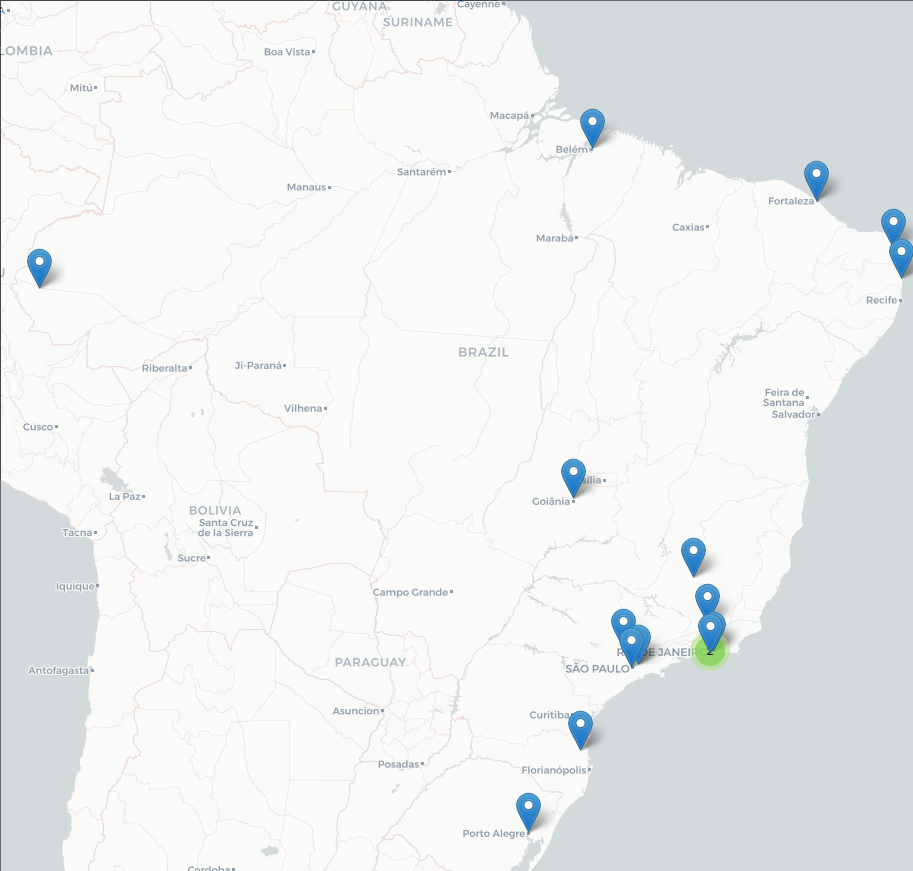
\includegraphics[width=.9\linewidth]{./img/labs-do-brasil.png}
\caption{Uma visão dos laboratórios e pesquisadores em psicolinguística no Brasil. Confira o mapa no \href{https://igordeo-costa.github.io/about/}{github.com}}
\end{figure}

\section{Proposta inicial}
\label{sec:orgafc0a60}

Elaborar uma plataforma \emph{online} em que os diversos laboratórios e pesquisadores do Brasil possam disponibilizar experimentos a fim de divulgá-los mais amplamente, para fora dos círculos das próprias universidades. Nessa plataforma, os pesquisadores cadastrariam seus experimentos com um pequeno texto descritivo (ver modelo anexo) bem como um link para que sejam acessados. Os diversos laboratórios, grupos de trabalho, programas de pós-graduação e pesquisadores, então, poderiam se vincular à plataforma como membros. Semanalmente, a plataforma divulgaria um boletim informativo a todos os membros com os experimentos que estão ali cadastrados. Os experimentos poderiam ser agrupados por áreas e/ou subáreas no momento do cadastro, de modo que os membros poderiam fazer divulgações mais direcionadas para determinados interesses. Por exemplo, um professor que deseje fazer um trabalho sobre orações relativas com os alunos, poderia, antes, pedir para que eles realizassem uma tarefa online e, a partir da tarefa, discutir questões pertinentes com os alunos. Desse modo, tenderia a haver maior engajamento na atividade.

\subsection{O que será disponibilizado}
\label{sec:org2a39bf9}

A plataforma não hospederá o experimento (como o faz o PCIbex, por exemplo), mas apenas o link que direciona ao experimento.

\subsection{Divulgação}
\label{sec:org29edcd1}

Os pesquisadores e laboratórios interessados cadastrarão seus e-mails e, quando um experimento for cadastrado na plataforma, receberão semanalmente um boletim informativo dos experimentos da semana.

Alunos e pessoas interessadas em serem voluntários como participantes também poderão cadastrar seus e-mails de modo a receberem, eles próprios, a divulgação.

\subsection{O que é preciso para cadastrar um experimento}
\label{sec:org43eb102}
\subsubsection{Termos técnicos}
\label{sec:orgc0c2f00}
\begin{enumerate}
\item Pesquisador responsável
\item Orientador (se mestrando, doutorando ou aluno de IC)
\item Laboratório a que está vinculado
\item Universidade a que está vinculado
\item Protocolo de Aprovação por Comitê de Ética apropriado
\end{enumerate}

\subsubsection{Participantes potenciais}
\label{sec:org826be4e}
\begin{enumerate}
\item Existe alguma limitação sobre quem pode realizar o experimento?
\end{enumerate}

\subsubsection{Divulgação}
\label{sec:org6721649}
\begin{enumerate}
\item Texto curto de divulgação do experimento
\item Link para acesso ao experimento
\end{enumerate}

\subsubsection{Exemplo}
\label{sec:orgf640a11}
\begin{quote}
Os pesquisadores Fulana de Tal e Cicrano de Tal da Universidade Estadual X do Laboratório Y te convidam para participar do experimento chamado “Leitura Autocadenciada de Blablabla”.

O experimento psicolinguístico envolve a leitura de frases a fim de verificar a sua interpretação sobre elas. Ao participar você contribuirá com o avanço do nosso entendimento de como a língua funciona.

Ficou interessado? Clique no link abaixo para saber mais:
\begin{itemize}
\item Link
\end{itemize}

(Idealmente uma imagem ilustrativa.)

Protocolo do experimento no Comitê de Ética número 000.
\end{quote}

\section{Com quem falamos a respeito?}
\label{sec:org88b2fe6}
\subsection{{\bfseries\sffamily TODO} Interessados [100\%]}
\label{sec:org690d839}
\begin{itemize}
\item[{$\boxtimes$}] Ana Paula Jakubów (Ex-UERJ; LAPAL/PUC-Rio)
\item[{$\boxtimes$}] Mercedes Marcilese (NEALP/UFJF)
\item[{$\boxtimes$}] Thiago Motta (LAProS/UNICAMP)
\item[{$\boxtimes$}] Renê Forster (UERJ)
\item[{$\square$}] Marina Maia (Doutoranda/Unicamp)
\end{itemize}

\subsection{{\bfseries\sffamily TODO} Potenciais interessados [0\%]}
\label{sec:org8c6fbc7}
\begin{itemize}
\item[{$\square$}] Érica Rodrigues (LAPAL/PUC-Rio)
\item[{$\square$}] Mahayana Godoy (UFRN)
\end{itemize}

\section{Afazeres [0\%]}
\label{sec:org503bbe4}
\begin{itemize}
\item[{$\square$}] Definir os interessados em contribuir para a elaboração do projeto
\item[{$\square$}] Finalizar a proposta
\item[{$\square$}] Criar o mapa de estágios do projeto
\begin{itemize}
\item[{$\square$}] Estágio 1: Divulgação para programas de pós e indivíduos
\item[{$\square$}] Estágio 2: Divulgação em redes sociais
\item[{$\square$}] Estágio 3: Implementação dos experimentos itinerantes
\item[{$\square$}] Estágio 4: …
\end{itemize}
\end{itemize}
\end{document}
